\documentclass[sigconf]{acmart}

\usepackage{booktabs} % For formal tables


% Copyright
%\setcopyright{none}
%\setcopyright{acmcopyright}
%\setcopyright{acmlicensed}
\setcopyright{rightsretained}
%\setcopyright{usgov}
%\setcopyright{usgovmixed}
%\setcopyright{cagov}
%\setcopyright{cagovmixed}


% DOI
\acmDOI{10.475/123_4}

% ISBN
\acmISBN{123-4567-24-567/08/06}

%Conference
\acmConference[CASES 2017]{International Conference on Compilers, Architecture,
and Synthesis for Embedded Systems}{October 2017}{Seoul, South Korea} 
\acmYear{2017}
\copyrightyear{2017}

\begin{document}
\title{Read Only Data Specific Management for an Energy Efficient Memory System}
\titlenote{Produces the permission block, and
  copyright information}
\subtitle{Extended Abstract}
\subtitlenote{The full version of the author's guide is available as
  \texttt{acmart.pdf} document}


\author{Gregory Vaumourin}
\affiliation{
  \institution{CEA LIST}
  \city{Gif sur Yvette} 
  \state{France} 
  \postcode{F-91191}
}
\email{gregory.vaumourin@gmail.com}

\author{Denis Barthou}
\affiliation{%
  \institution{INRIA Bordeaux Sud-Ouest, LaBRI}
  \streetaddress{Institute of Technology}
  \city{Bordeaux} 
  \state{France} 
%  \postcode{43017-6221}
}
\email{denis.barthou@inria.fr}


\begin{abstract}
This paper provides a sample of a \LaTeX\ document which conforms,
somewhat loosely, to the formatting guidelines for
ACM SIG Proceedings.\footnote{This is an abstract footnote}
\end{abstract}

%
% The code below should be generated by the tool at
% http://dl.acm.org/ccs.cfm
% Please copy and paste the code instead of the example below. 
%

 \begin{CCSXML}
<ccs2012>
<concept>
<concept_id>10010520.10010521.10010528.10010536</concept_id>
<concept_desc>Computer systems organization~Multicore architectures</concept_desc>
<concept_significance>500</concept_significance>
</concept>
</ccs2012>
\end{CCSXML}

\ccsdesc[500]{Computer systems organization~Multicore architectures}
\ccsdesc[500]{Computer systems organization~Embedded systems}

\keywords{cache, read-only}


\maketitle

\section{Introduction}

Caches are widely used in modern processors to effectively hide the data access latency since memory reference patterns in most applications have good spatial and temporal locality. But with the number of cores increasing, adopting hardware-controlled caches increases the energy consumption for two reasons. The automatic data management in caches is costly and the coherence protocols do not scale very well with the number of cores. As reported in the literature, the cache hierarchy consumes between 25\% and 50\% of the energy of the chip~\cite{Segars:2001} on current systems. With the growing focus on energy efficiency, it is important to find ways to reduce energy without sacrificing performance


We can found two main motivations for heterogeneous management that lead to different classifications inside the memory system.

First, a group of solutions tries to classify data based on their locality property. Different types of data between instruction, head data, stack data, and global data have different locality properties and cache uses and specific cache structure can be build for each type. This type of solution has been studied with success since the early days of cache memories. In the 60s, Harvard architectures separate the L1-level cache into instruction cache and data cache. In 90s, Gonzalez and al.\cite{Gonzalez:1995} proposed to go further in this direction with a data cache organization that separate data with high temporal locality (temporal cache) from data with spatial locality (spatial cache). The \textit{Region-based caching} introduced by Lee and al\cite{Lee:2000} decomposes the data cache into even more specialized structures, one structure for each kind of data: global data, stack data and heap data. These propositions has been improved since their first proposition but it illustrates the idea that such hardware-based solutions open up degrees of freedom for cache design and cache optimization. They bring important energy consumption reduction if the separation of data results in two sub-groups of data with very different cache uses. The difficulty of such organization is to be able at hardware level, to determine the type of accessed data and drive the request to the relevant sub-memory.

A second group of solutions optimizes coherence protocols by classifying data between Shared and Private, and Read-Write and Read-Only. Indeed, some analysis shows that the amount of data that required to be watched by costly coherence protocol is actually   
The goal is to isolate a specific property of the data in order to improved 

We propose in this paper 

In both group of solutions, 

Understanding 

In industrial work, the Kepler architecture~\cite{NVIDIA:2007} for NVIDIA GPUs offers a read-only cache as an improvement of the previous texture cache. Using this cache can remove loads and reduce the size of the shared L1 working set. It can be use automatically by the compiler or explicitly by the user. We study in this paper the pertinence of such idea for cpu-based architectures.

A previous study~\cite{vaumourin:2014} performed on a standard set of applications for embedded systems reveals an important difference of behavior between read-only data and read-write data in terms of reuse and memory access distribution, especially for image processing applications. The study show that the difference of behavior between read-only and read-write data is important enough to consider specific management of these data. It improves the locality and cache use on both sub-set of data. Specific management for a particular kind of data opens degrees of freedom for cache designs which have an important impact on energy consumption. Moreover, specific optimization for such datapath can also be explored. The contributions of the paper are the following: an illustration of the difference of behavior between read-only and read-write data, the description of a data classification methodology at compile time, an empirical architectural exploration for the specific management of the read-only data into a generic memory system. The experimental evaluation shows that the final solution with specific read-only data management can decrease the energy consumption of the memory system by 20.6\% on average without performance penalty on a set of multithreaded image processing benchmarks. The data classification at compile-time performs a detection rate of 89,3\% in average compared to an offline analysis. The organization of this paper is the following: Section II justifies the specific behavior of read-only data in terms of data locality. Section III details the compile-time data classification. Section IV highlights our architecture exploration methodology and the evaluation methodology. Section VI describes the experiments results. Section VII study a specific optimization for the read-only datapath. Finally, Section VIII provides our conclusions.


\section{Read-only Data Characterization}

As mentioned before, the specific management in the memory system for a particular kind of data has been successfully studied in the past. These solutions creates two sub-groups of data with very different needs and use of cache memory. This difference is often intuitive like the difference of behavior in the memory between data and instructions. For read-only data, this difference needs to be illustrated first by a detailed study before considering specific management.  

We define read-only data as data used in a read mode either for the
whole application execution (input data) or for a more limited scope
such as a function, a kernel or a loop. In this case, read-write data
can switch into read-only mode for some scope and then switch back to
read-write mode. Our analysis is mostly focused on image processing
applications, since these applications are often implemented as
a pipeline of tasks where the output (written) data of a task
corresponds to the input (read) data of the next one. Such computations
manipulate large regions that are in a read mode on a long scope.

We study the separation of the memory stream with a data locality metric: the reuse distance~\cite{Coffman:1973}. This metric is defined as the number of different accesses between two accesses to the same address and depends only on the cache block size (fixed to 64B). A two-step analysis is followed: First, a memory trace is extracted from an instrumented execution of the analyzed application. Then, the read-only data and read-only periods are detected through an analysis of the memory trace. This offline analysis explores the trace in a 2D space (time and address) to detect rectangular areas solely composed of read accesses. Such analysis is manually tuned to detect read areas in an adequate grain in order to avoid capturing every read access as a small read-only area. The main memory trace is then split in read-only and in read-write traces. The average reuse distance is computed on all traces: The original trace and the 2 sub-traces. The results, shown in Figure \ref{stackdistance}, are normalized to the average reuse distance of the full trace.


\begin{figure}
    \centering
    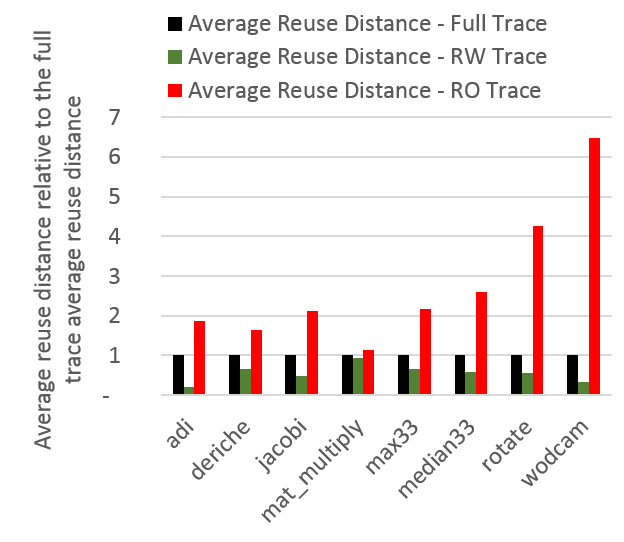
\includegraphics[width=8cm]{./images/stackdistance.png}
     \caption{Variation of the average reuse distance}
    \label{stackdistance}
\end{figure}

On all the evaluated benchmarks, two important observations can be made: the average reuse distance of the read-only data is 8.4 times bigger than the reuse distance of the read-write stream and removing the read-only data from the main memory stream reduces the average reuse distance by 32\% in average. The read-only data present much less data locality than average data and they can create potentially more pollution into the cache hierarchy. Removing them from the main memory stream flow therefore enhances data locality of the main memory flow and leads to better cache use. This conclusion has been extended to the standard set of benchmarks Mibench~\cite{vaumourin:2014} and similar conclusions can be drawn for image and signal processing applications. 


\begin{figure}
    \centering
    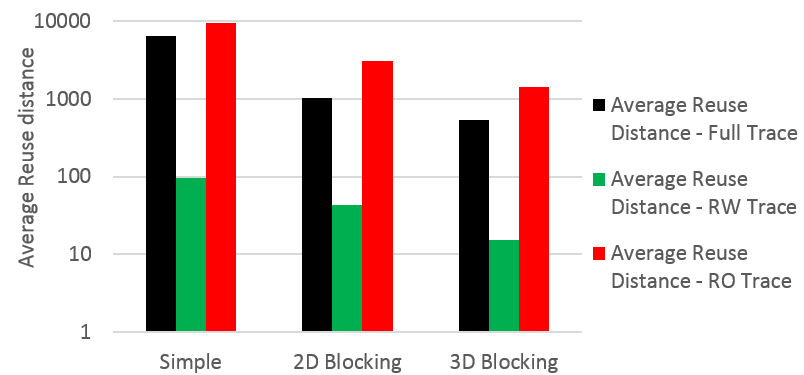
\includegraphics[width=9cm]{./images/blocking1.png}
     \caption{Average reuse distance with several tiling strategies}
    \label{blocking}
\end{figure}

Read-only data detection and reuse distances depend heavily on parameters such as the degree of locality optimization applied to source code or input data sizes. As an example of locality optimization, the tiling is studied on the \textit{matrix\_multiply} benchmark. Figure \ref{matmul} shows 2D and 3D tiling transformation applied to \textit{mat\_mult} and different tile shapes are evaluated. The tile shape with the best result in terms of average reuse distance of the full trace is kept for the results of Figure \ref{blocking}. In this case, tiles parameters are K=8,J=32 for 2D tiling, and K=8,J=16,I=1 for 3D tiling. It shows that even though the average reuse distance varies with the applied transformation, the average reuse distance between the sub-memory streams remains at the same level. This locality difference comes from the algorithm structure. The read-only matrix accessed in column-order, produces long reuse distances compared to the other, tiling can reduce this distance but will always be larger than the output matrix that reuses its data between each iteration of the innner loop.  The conclusion drawn from the simple version of \textit{matrix\_multiply} stays valid with tiling transformation. However, some locality transformations such as loop fusion can create pathological cases for read-only data detection. For example, if a memory region is read in one loop body (creating a read-only period) and written in the other, merging the 2 loops would cancel the read-only period resulting in no detected read-only data. 

In another direction, the influence on the results of the input data sizes has been studied. Since our methodology uses memory traces, there are technical limitations to the amount of access. The working set size that we study stays at best one order of magnitude under classic working set size used in embedded system. However, several measure points have been taken with different input data size and the tendency of the results suggest that increasing the working set sizes increases the difference of the reuse distance illustrated Figure \ref{stackdistance}, reinforcing our conclusions. The illustrated difference of data locality between read-only and read-write data, motivates the idea of a specific management. The next section studies a data classification mechanism at compile-time in order to place the read-only data in the right data path. 

\begin{figure}
    \centering
    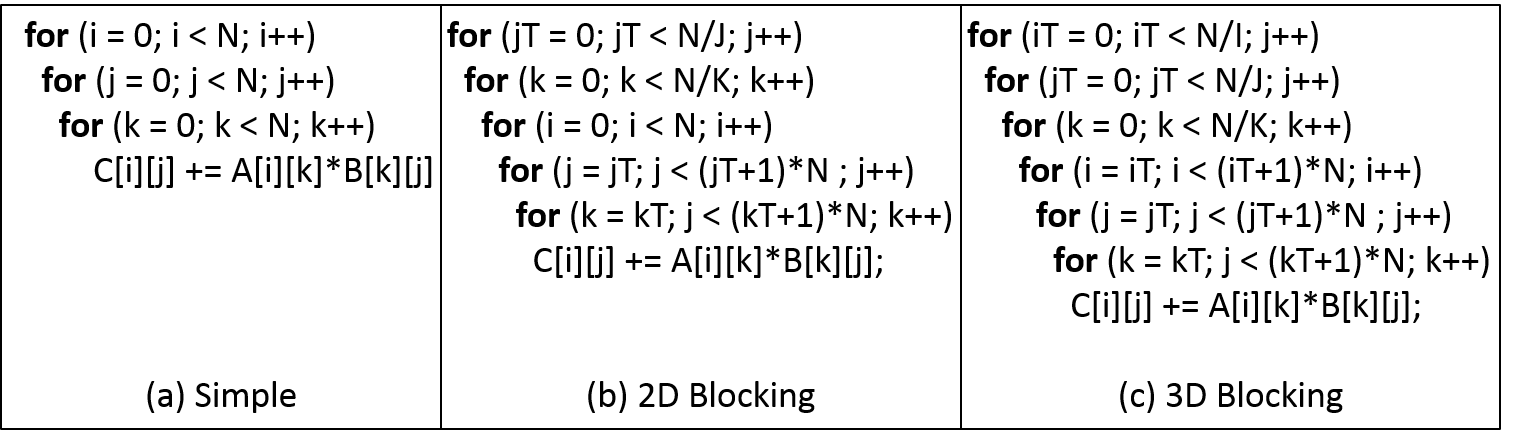
\includegraphics[width=9cm]{./images/matmul.png}
     \caption{Evaluated tiling strategies for \textit{mat\_mult}}
    \label{matmul}
\end{figure}


\section{Read-only data Detection}

In the literature, examples\cite{Cuesta:2013}\cite{Pugsley:2010} of read-only data classification can be found at hardware-level for coherence optimization purpose. These solutions mostly detect read-only data at page granularity in a reactive fashion. A page is first considered read-only and a single write on the page switches the status of the page into read-write mode. Compared to a block granularity detection, Page granularity can produce poor detection rates and leads to under-optimal solutions. On the evaluated applications in \cite{Cuesta:2013}, the detection rate of read-only data goes from under 40\% to more than 60\% when switching from page to block granularity. Moreover, hardware-based proposition are area-constrained and limited to simple detection methods such as saturation counters. We propose here a mechanism for read-only data classification at compilation stage. Our solution relies on existing dataflow techniques to reach high detection rates and allow data classification at cache block granularity. 

\subsection{Static Analysis}

The goal of dataflow analysis performed by the compilers is to retrieve information about the handled data to perform some optimizations.

For scalar analysis, definition-use chains (DU chains) link the definition (write operation) to all corresponding uses (read operation), they are standard data structures constructed by the compiler.
This information can be directly reused for the detection of read-only periods of scalar variables. For pointers, arrays and structures, we developed an extension of the alias analysis as an intra-procedural pass that focuses on nested computational loops. The algorithm is the following. For each loop, the pass iterates over the loop body, and maintains two lists of memory references, a read-only and a read-write list. These lists are then built for each loop nest. The results of alias analysis help us correlates the memory reference to memory regions. In order to consider a memory region as read-only, all references that points to the region must come from the read-only list. The status of memory regions can then be deduced for each loop nest and this property can vary between loop nests. The analysis uses a conservative approach in order to ensure that every reference captured is read-only. For example, if there are conditional branches in loops, the memory region needs to be read-only in all the paths in order to be considered read-only. Also, as the abstraction we use for memory regions is an interval, entire intervals are considered to be either read-only or read/write. 



\begin{figure}
    \centering
    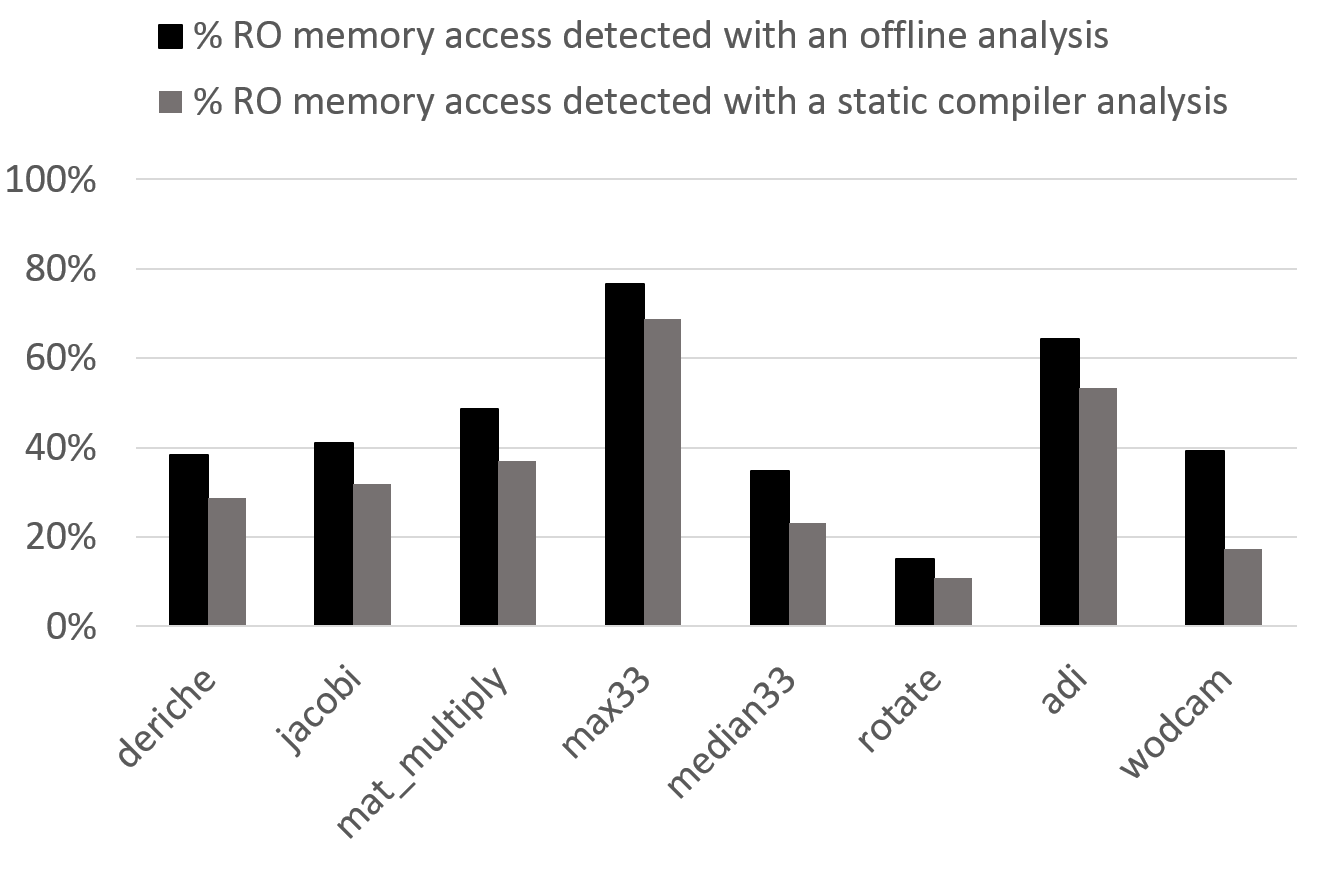
\includegraphics[width=8cm]{./images/plugin_result.png}
    \caption{Comparison between the read-only memory accesses detected with offline analysis and with the static analysis}
    \label{comparAcces}
\end{figure}

This algorithm has been implemented as a GIMPLE pass in GCC 4.9. To determine the quality of this static analysis, the results are compared to the exhaustive offline analysis presented Section II. Results in Figure ~\ref{comparAcces} show the static analysis we propose is able to capture most of the read-only memory accessed compared to the offline analysis. The detection rate is 89.7\% in average for the considered applications compared to the offline analysis, which is suitable to consider architectural specific management. 

The static analysis developed is fairly simple compared to existing dataflow analysis present in compiler but it highlights the fact that read-only information is quite simple to extract from a compiler. Therefore, compile-time read-only data detection is pertinent and can be part of a co-designed architecture that proposes specific management for read-only data. The detection rate suits our requirements for the analyzed applications and in case of more complex applications, more complex analysis can be used such as inter-procedural dataflow analysis to study accessed memory regions. 

\subsection{Considerations}
Position de la passe dans le flow d'execution 


\subsection{Compiler-Hardware Interface}

The solution assumes that each processor knows the datapath to use
when accessing a given cache block. We propose to add this information
directly into memory request, this technique is known as a cache
collaborative technique or cache hints. Existing architectures already use these kinds
of extra bits in the instruction, such as the prefetch and evict-next
instruction in the Alpha 21264 	
We believe that, in most architectures, the increasing speed gap between memory and
processor will justify the inclusion of additional bits in the
instruction code to facilitate the reduction of this gap.

The benefits are twofold: It allows to work on block granularity
classification that is proven to be important for the detection rate
and it allows to transfer semantic information dependent on the code and
independent on the execution context.

\section{Architecture exploration}

This section describes the architectural exploration of read-only data
specific management. A specific cache is added along a classic
cache-based memory system to handle specifically the read-only memory
accesses. The exploration focuses on two aspects: the level of memory
where it is pertinent to add the read-only cache (RO cache) and the
shared/private property of this cache. Starting from a generic memory
hierarchy of two levels with private first level caches and shared
unified last-level cache (LLC), it creates three architectural
possibilities presented Figure~\ref{architecture} which describes
three scenarios. Since the read-only property of the data is dynamic,
data can be accessed by both data paths depending on the time of the
execution. Switching technique between data paths must then be
considered in order to avoid coherence issue between the read-only
(RO) cache and the RW cache of the same level. The resolution of this
problem can incur overheads if a cache line has to do many switches
between  RO and  classic data paths because we do not consider
direct transfer between caches of the same level in this work.


\begin{figure}
    \centering
    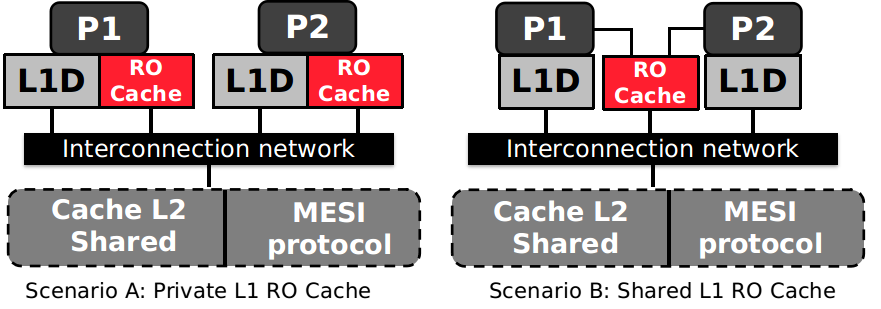
\includegraphics[width=9cm]{./images/architecture.png}
    \caption{Overview of cache design methodology for specific read-only data management}
    \label{architecture}
\end{figure}

\subsection{Scenario A}

The first scenario considers a private RO cache for each core. This solution is similar to the separation of the instruction cache and data cache. In this case, a cache line cannot be in the two caches so the L1D-cache and RO cache are mutually exclusive. If a cache line, present in one of the cache, needs to be accessed by the other cache, it needs first to be invalidated and eventually written back to the L2 if modified. Each entry of the sharer list in the L2 cache has a additional bit to store the location of the block (L1D or RO cache). 

\subsection{Scenario B}

The scenario B considers a shared RO cache across all processors. This situation is similar to Kepler architectures in NVIDIA GPUs~\cite{NVIDIA:2007} in which the read-only cache is shared across a whole warp. The coherence problem is resolved in this case by using the same MESI coherence state machine for RO cache as for L1D cache. From the coherence protocol point of view, it is equivalent to have a fifth L1D cache to track. Note that in our simulations, the RO cache is not multi-ported because this increases prohibitively the cost per access which is not suitable for a cache close to a processor. Instead, the requests are sequentialized into a FIFO buffer and a processor may has to wait for another processor to finish its request before being serviced by the read-only cache.


\subsection{Scenario C}
The last scenario considers a read-only data management at L2-level. In this case, the L2 RO cache is shared across cores but the coherence problem is more difficult to solve. For each access, the cache line at L1-level is tested for its status, encoded in one bit. If there is a status switch, the L1 controller warns the corresponding L2 cache that informs L1 cache sharing the cache line to update their status. Then a switch of the cache line at L2-level is operated between L2 and L2RO (depending on the status modification). During the switch, the L1 cache lines are not invalidated but this operation stalls the memory system in order to guarantee that the coherence of the system is preserved. As in scenario A, the L2 and RO caches are mutually exclusive. All these architecture possibilities introduce an overhead in their management due to cache line switching. Our conviction is that this overhead stays small because the read-only regions captured by the compiler are on large loop nests, the granularity of the detected RO memory regions is supposed to be large enough to bring few status switches.

\subsection{Evaluation}

\begin{figure}
    \centering
    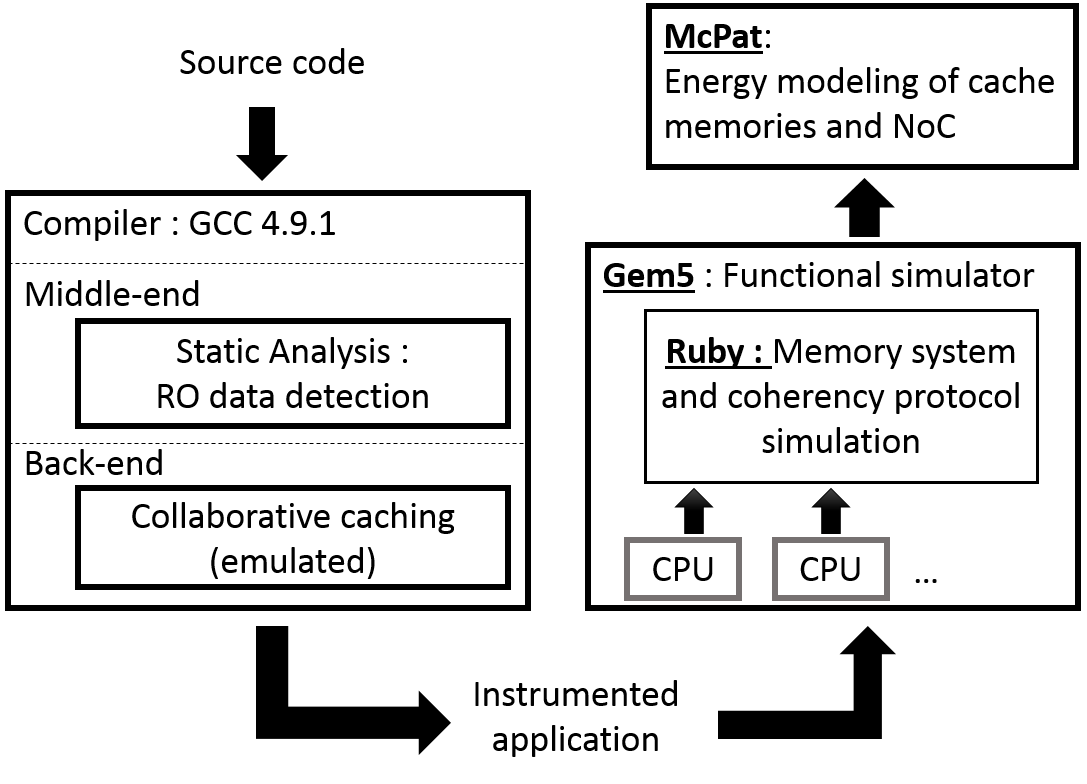
\includegraphics[width=8cm]{./images/workflow.png}
    \caption{Simulation Workflow}
    \label{workflow}
\end{figure}

For our experiments, we use the Gem5 simulator~\cite{Binkert:2011} to
implement our architecture proposition, with the sub-simulator Ruby to
describe the memory system and the coherence protocol. It allows
detailed simulation of the cache hierarchy. The energy consumption of
caches and interconnection network are obtained from the McPat
framework v1.3~\cite{Li:2009}. To mitigate simulator errors, results
are always presented in relative difference. The overall workflow is
represented in Figure \ref{workflow}. The baseline system
configuration is shown in Table~\ref{designs}. For each scenario, two
sizes for the read-only cache are considered
% because size is the most sensitive parameter for cache design.  
The additional storage needed for read-only cache is compensated by
reducing the size of the L2 cache. The size of the L2 is reduced by
removing its necessary amount of ways. Table~\ref{sizesCaches}
describes the balancing of the storage between the L2 and the
read-only cache. Note that the area taken by cache controllers are not
considered, meaning that the comparison is storage-constant and not
strictly area-constant.

\begin{table}
\centering
%\normalsize
\caption{Constant system parameters during simulations}
\label{designs}
\begin{tabular}{ | c | c | }
\hline
\hline
 & System Parameters \\
\hline
CPU & 4 cores in-order, 1GHz, 1 load/store unit\\
\hline
L1-D cache & 32KB, 2-way assoc., 64B blocks, LRU\\
\hline
Local Network& Crossbar , 64B wide, 2 cycles lat.\\
\hline
DRAM  & 512MB, 1 memory channel at 12.8GB/s\\
\hline
\hline
\end{tabular}
\end{table}


%Expliquer les differentes propositions d'architectures au niveau des tailles de caches (pas les assoc) , les locked ways L2 
\begin{table}
\caption{L2 and read-only cache storage Allocations for every scenario exploration}
\label{sizesCaches}
\begin{tabular}{ |c|c|c|c|c|c|c|c| }
\hline
\hline
% & Baseline & Scenario & Scenario & Scenario & Scenario & Scenario & Scenario\\
 &Baseline   & A & A & B & B & C & C\\
\hline
 Cache RO & - -  & 8kB & 16kB & 16kB & 32kB & 64kB & 128kB\\
      &  & FU & 2-way &  2-way & 2-way & 2-way &  4-way \\
\hline
 Cache L2 &  256kB & 224kB & 192kB & 224kB & 224kB & 192kB & 128kB \\
  &  8-way & 7-way & 6-way  & 7-way  & 7-way & 6-way & 4-way \\
\hline
\hline
\end{tabular}
\end{table}

\section{Results}

\subsection{Benchmark Description}

All benchmarks are presented in Table~\ref{benchs}. They come from in-house set of benchmarks and are written in C, parallelized with OpenMP and compiled with the presented plugin and \texttt{O3} optimization. Most of them are taken from image processing domain and no locality transformation has been used. We compare the efficiency of the proposed solutions, the main focus is the energy reduction of the system while keeping performance. The performance of the system is measured through the AMAT metric (Average Memory Access Time) because all other parameters (branch predictions, computation, ...) are constant between simulations. The energy consumption, the AMAT and the misses at L1-level are shown in Figure~\ref{results} for the different scenarios. Note that the RO cache misses are counted as L1-level misses for scenarios A and B.

\begin{table*}
\centering
\caption{Benchmarks description}
\label{benchs}
\begin{tabular}{ |c|c|c|c| }
\hline
\hline
  Benchmarks &  Input Data & Description &  \% of detected  \\
   &  &  &RO accesses \\
\hline
 matrix\_multiply & 512x512 arrays&  Blocked version of matrices multiplication& 37.0\%\\ 
\hline
 deriche & image of 1024x1024px& Canny edge detector algorithm& 28.6\%\\
\hline
 rotate & image of 1024x1024px &  Rotation algorithm of an image & 10.8\%\\
\hline
 max33 &  image of 1024x1024px & Average blur algorithm of an image& 68.8\%\\
\hline
 median33 &  image of 1024x1024px& Median algorithm of an image& 23.0\%\\
\hline
 jacobi & 1024x1024 matrices  &Iterative algorithm that computes the solutions of a system of linear equations & 37.0\%\ \\
\hline
 adi & 256 elements arrays (10 iterations) &  Algorithm for solving non\-linear differential equations & 53.3\%\\
\hline
 wodcam & 1000 test images (168x192px) &Recognition faces application based on eigenface method & 17.6\%\\
\hline
\hline
\end{tabular}
\end{table*}

 
%\begin{figure}
%    \centering
%    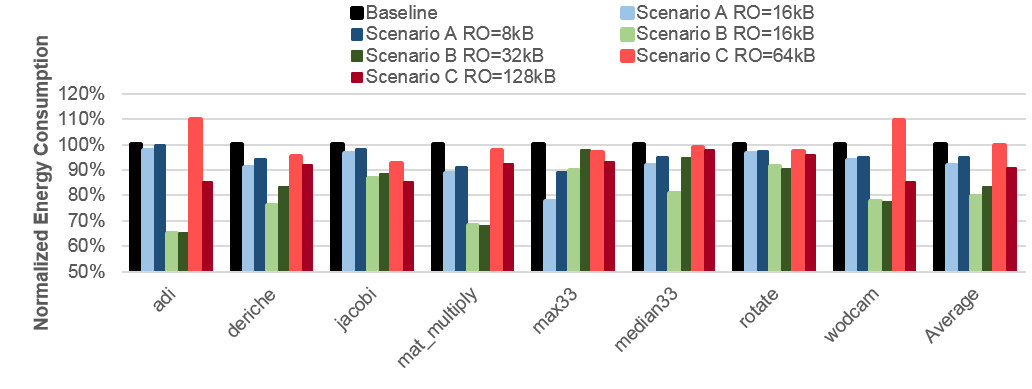
\includegraphics[width=12cm]{consoResults.png}
%    \caption{Normalized energy consumption variation of the architectural propositions}
%    \label{consResults}
%\end{figure}
%
%\begin{figure}
%    \centering
%    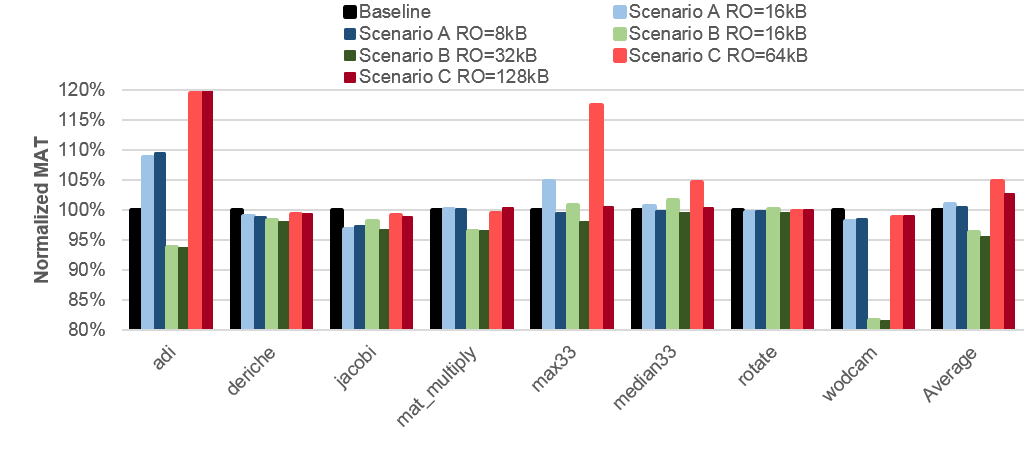
\includegraphics[width=12cm]{perfsResults.png}
%    \caption{Normalized AMAT variation of the architectural propositions}
%    \label{perfsResults}
%\end{figure}

%\begin{figure}
%    \centering
%    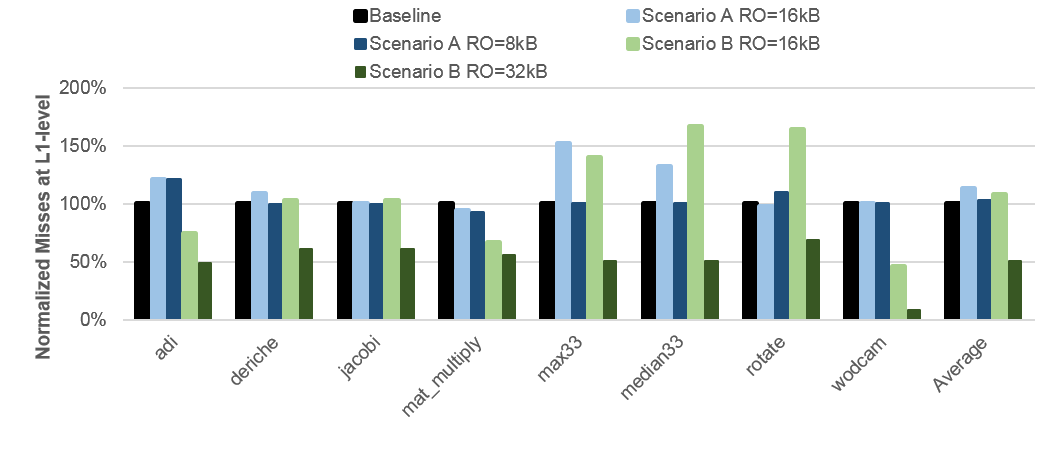
\includegraphics[width=12cm]{missResults.png}
%    \caption{Normalized miss variation at L1-level for scenario A and B }
%    \label{missResults}
%\end{figure}
\begin{figure*}
    \centering
    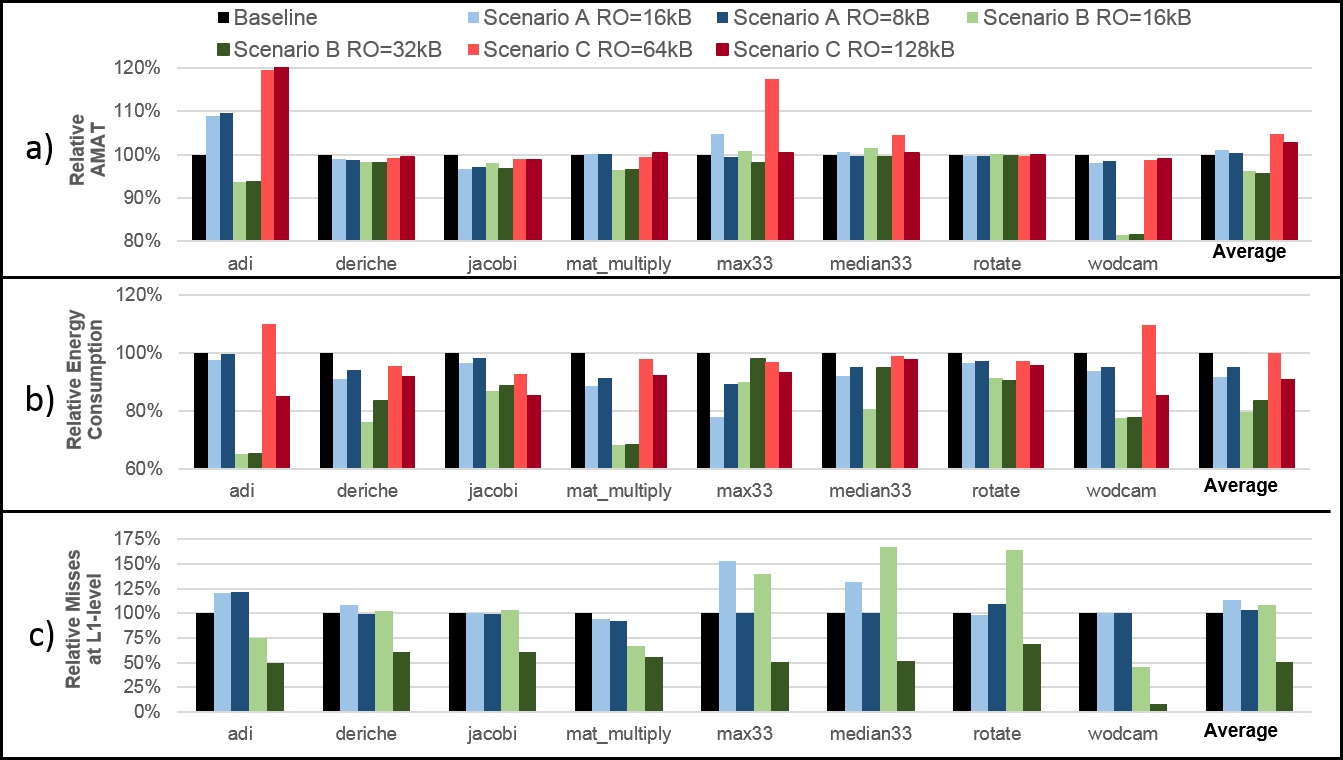
\includegraphics[width=15cm]{./images/results.png}
    \caption{a) Normalized AMAT (Average Memory Access Latency) variation and b) Normalized energy consumption variation of the architectural propositions. c) Normalized miss variation at L1-level for scenario A and B}
    \label{results}
\end{figure*}


\subsection{Scenario A}

In scenario A, the number of cache misses stays relatively similar to the baseline even if the miss rate of L1D caches is decreased by an average of 17.56\%. As anticipated by the result of Section II, the locality of the main memory stream is improved when the read-only stream is removed. Note that this depollution of the L1-D caches is observed in the same proportion in scenario A and B. The number of misses does not change significantly because misses occuring previously on the L1D are now on the RO cache. Read-only accesses represent only 28.5\% of the total memory access in average, and they are divided equally between the 4 cores. In this case, private read-only caches handle very few memory accesses and yet are not able to resolve misses. This negates the performance improvements on L1D-caches and points out the poor use of the RO cache resources. The small energy improvement in this proposition is based on the fact that the read-only accesses are handled in a smaller cache than the baseline, the energy cost per access is lower.
% In this case, one can think of a different cache policy than LRU to handle the RO cache that consider a stream with few reuse

\subsection{Scenario C}

Placing the specific management at L2 level brings few energy reduction and no performance gain. Generally, less reuse occurs at L2-level than at L1-level. Dividing the memory stream at L2 level breaks this reuse and creates a prohibitive increase of the number of accesses to the main memory: +46\% for 128kB L2RO case and +70\% for 64kB L2RO case in average. The system spends time and energy due to an inefficient way to switch cache lines between the two L2 caches that has to transit through main memory. One may propose a better mechanism or a cache partitioning technique in this case, such as proposed by Khan and al.\cite{Khan:2014} to improve this solution. 

\subsection{Scenario B}

Scenario B presents a great cache miss reduction for a 32kB read-only
cache and the best energy improvement of 20.6\% in average. With a RO
cache of 16kB, the miss reduction is not as important but, due to a
cheaper cost per access, this miss reduction that occurred for a 32kB
RO cache is converted into energy savings because of a more aggressive
cache design.
%which leads to important energy improvements. 
Generally a shared cache implies a better use of resources but
can provoke destructive interferences in the cache or performance
degradation because of the resource contention. Since read-only
accesses represent only 28.5\% of the total memory accesses and the
great improvement in term of cache efficiency, the negative effects on
performance stay marginal. The miss penalty observed for \textit{rotate},
\textit{max33} and \textit{median33} can be explained by the fact that
the baseline of these benchmarks is already very efficient, the miss
rate at L1-level stays under 1\% and most of the cache misses
are compulsory misses, that cannot be improved by the proposed architecture. The additional cost caused by the miss increase is
largely compensated by smaller cost per access for the read-only cache
in these cases. \textit{adi} and \textit{mat\_multiply} show an
important miss reduction at L1-level even for a 16kB RO cache, because
most of their read-only working set are shared. In these cases,
processors are able to share the same cache block directly at L1-level
into the RO cache. Such phenomena decreases the reuse distance of this
block. The solution greatly benefits from this
application characteristic. Scenario B with a RO cache of 16kB is
the best for energy improvement and further analysis on this scenario
is performed in the following sections.

\subsection{Impact of the RO cache latency}

Concerns can be made about the performance results presented
previously for Scenario B. During the experimentations, the RO cache
is configured to have the same latency as a classical L1-D cache
because they are logically on the same level. In a real system, the RO
cache latency would be larger than the L1D cache latency because it is
shared across cores. Moreover, the L1RO latency is critical because it can potentially stall all
processors. Some additional experiments have been made in
order to study the impact of the latency of the RO cache on the
overall system performance. This latency have been varied from 3
cycles to 15 cycles. As a reminder, the latency of an L1D-cache is 3
cycles, for L2 cache, 15 cycles. From 3 to 15 cycles, the relation
between the latency of the RO cache and the average AMAT degradation
relative to the baseline is linear with the formula:
\centerline{$\%AMATdegradation = 1.55\% * ROLatency +0.91$}\\
So, each cycle added to the RO cache latency brings an average AMAT
degradation of 1.55\%. For a latency of 5 cycles, the AMAT degradation
is null compared to the baseline architecture. The 5\% degradation
barrier is crossed with a RO latency of 9 cycles. These results show
that performance degradation is observed only with really pessimistic
scenario.

\subsection{Scalability of the solution}
\begin{figure}
    \centering
    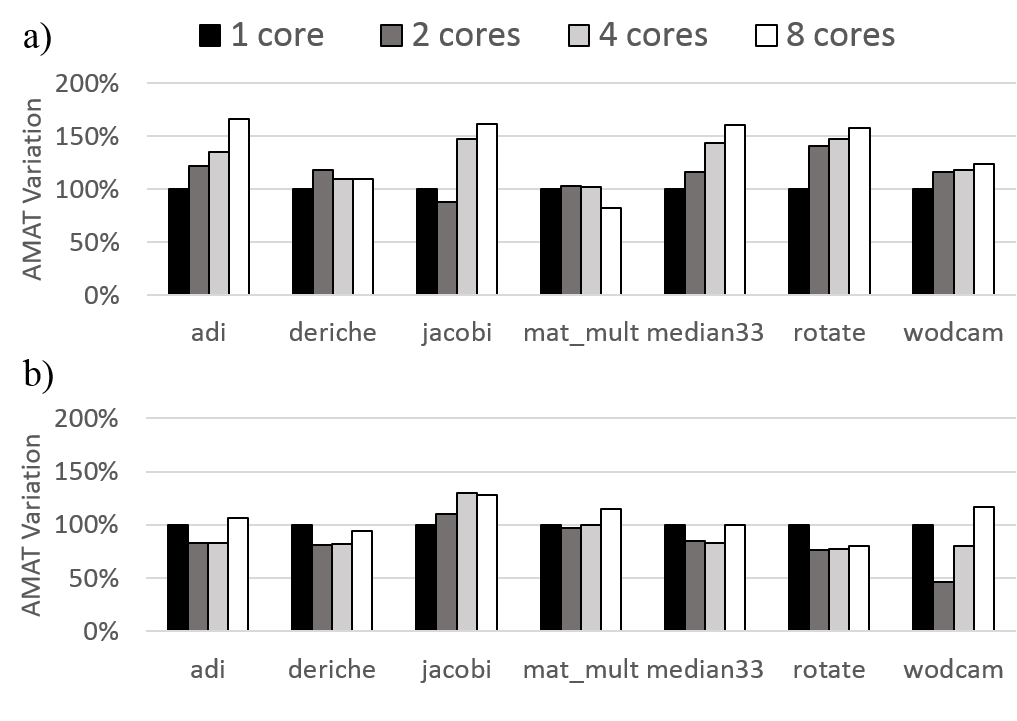
\includegraphics[width=9cm]{./images/scalabilityAMAT.png}
    \caption{For scenario B, AMAT variation of a) the RW datapath (L1D-L2) and b) RO datapath (Cache RO-L2) normalized to the unicore baseline}
    \label{amatVariation}
\end{figure}

We study the results of Scenario B regarding the strong scalability of the memory system. Figure \ref{amatVariation} shows the average AMAT for the two datapaths, normalized to the baseline unicore solution. As the number of cores increases, bank conflicts, contention on shared ressources (bandwidth and caches) and coherence protocol may impact performance of any of the datapath (RO and RW). Figure \ref{amatVariation} shows that the response time of the RW data path is essentially impacted by these destructive interferences. On the contrary, for the RO datapath, the AMAT stays relatively stable because increasing the number of cores increases the cache sharing effect, outbalancing the previous negative impacts. As the applications are parallelized with OpenMP and threads run on identical processors, threads run similar codes at the same IPC, so they tend to work on shared data at the same moment of the execution allowing reuse accross processors into the RO cache.

 
\section{Specific RO Cache optimization}

Adding more caches to the memory system increases the design complexity but also opens degrees of freedom for specific optimizations. This section explores one possible specific optimization for the RO cache based on the observation that it issues only read requests. This property is guaranteed by the conservative static analysis. No tracking is then needed from the coherence protocol in the same way as instruction cache. Such optimization is related to an important number of work from the literature proposing to reduce the impact of coherence by limiting expensive coherence mechanisms to shared read-write cache blocks. Several recent propositions~\cite{Cuesta:2013}\cite{Ros:2012}\cite{Davari:2015} classify data as private or read-only in order to reduce the coherence overhead and reduce directory design, this classification is done mostly at OS or hardware level. Such propositions are shown to improve the scalability of the architecture and reduce the energy consumption. Such solutions initialize all data status as private. When shared write accesses occurs, the status of the data (a whole page or a cache block depending on the solution) switches to shared and costly coherence recovery mechanisms are used to recover from this classification error. Moreover, such solutions usually do not consider transition back to the private status. Compared to such solutions, our proposition allows the status transitions of the cache block and does not need additional harware mechanism to protect against classification error as the compiler garantees the correctness of the classification. Our proposition of a shared read-only cache at the first level of hierarchy contributes as an orthogonal approach to such optimization that can include read-write data that present read-only periods into this optimization, increasing the scope of such optimization.\\
\indent The coherence state machine of the RO and L2 cache controller have
been modified in order to avoid the tracking of the read-only cache
blocks. The state machine of the read-only cache is very similar to an
L1D cache in a unicore system. Figure~\ref{incoherent} illustrates two
examples that benefit from a non coherent RO cache. In the first case,
a read request incurs a miss in the cache and a cache block needs to
be invalidated. The L1D cache has to inform the L2 cache about this
eviction even if the cache block is not modified, so that the L2
controller can update the sharers list. This property is required in
order to keep an inclusive system. This precaution is not needed with
the RO cache, resulting into several benefits. First, evictions from
the RO cache need less messages. Second, the system is not fully
inclusive anymore, as cache block can be evicted from the L2 cache and
kept into the RO cache without specific tracking, increasing
cache efficiency. The second example illustrates the fact that RO
cache operations do not change coherence state of the others
caches. Usually, a read request of a cache block that is already
modified in another L1D cache creates a costly downgrade transaction
of the cache block from Modified to Shared. With a RO cache, such
transaction requires less messages and no modification of the
coherence state of the cache block in the L1D and L2 caches. It means
that the L1D cache still has read/write permission to the cache block
after a read access from the RO cache, and potentially a future write
request will not miss. \\
\indent The state machine of a non coherent RO cache has been implemented into Gem5 and compared to the result with the coherent RO cache. As anticipated with the examples of Figure~\ref{resultIncoherent}, a non
coherent RO cache mainly reduces the network traffic of 26\% compared
to coherent RO cache, decreasing the energy consumption by 4\% in average compared to the results of the previous section. It can also
prevent the prohibitive increase of messages that occur for example on
\textit{median33} and \textit{max33} due to the L1 miss
increase observed for these applications with scenario B. But cache
efficiency stays relatively stable between the two scenarios. On the
evaluated applications, only \textit{adi} presents an important amount
of Modified->Shared transitions on L1D caches that benefit from the
non coherent read-only cache, in the same way as the situation
described in the latter case of Figure~\ref{incoherent}. For
\textit{adi}, cache efficiency is improved and significant gain on the
AMAT (17,6\%) and energy consumption (11,3\%) can be found compared a
solution with a coherent RO cache.

\begin{figure}
    \centering
    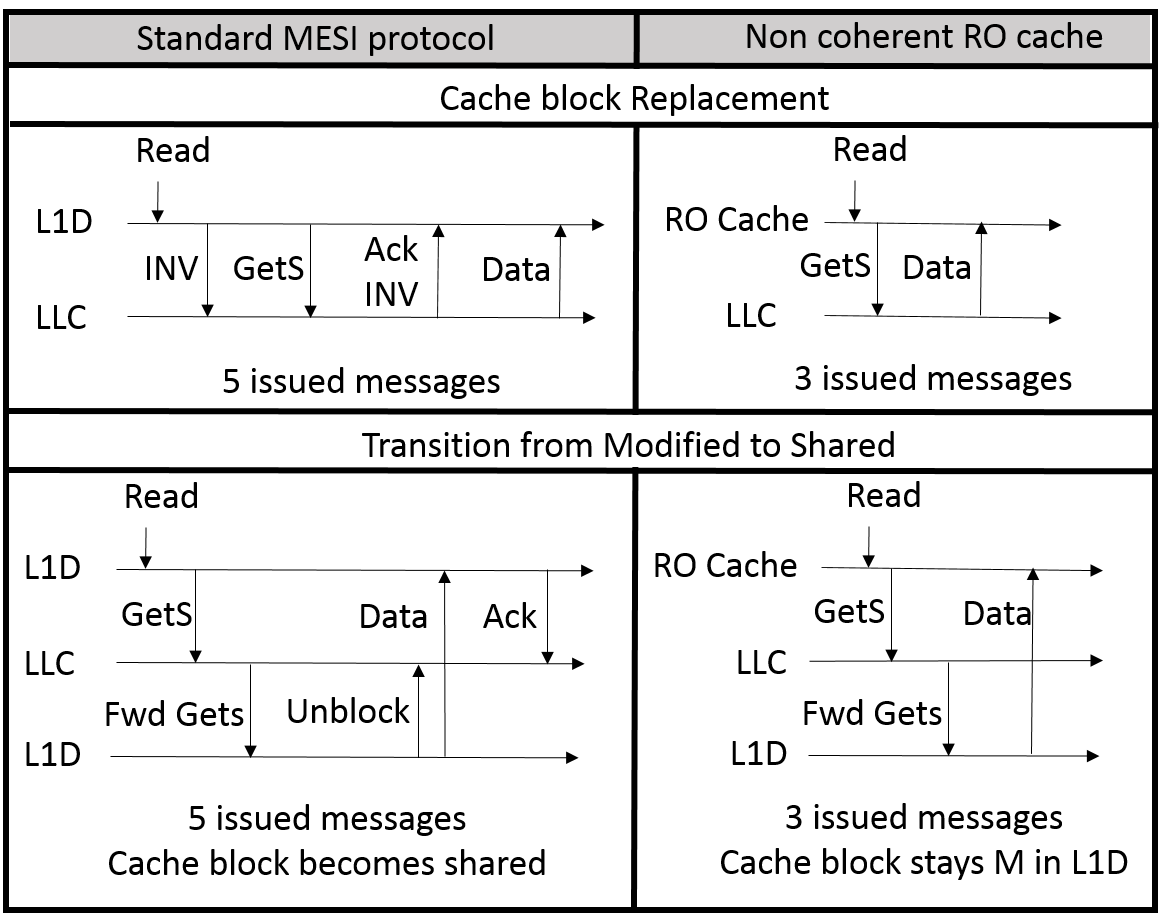
\includegraphics[width=9cm]{./images/incoherent.png}
    \caption{Difference of the procedure with non coherent RO cache during  cache block remplacement and downgrading operation}
    \label{incoherent}
\end{figure}


\begin{figure}
    \centering
    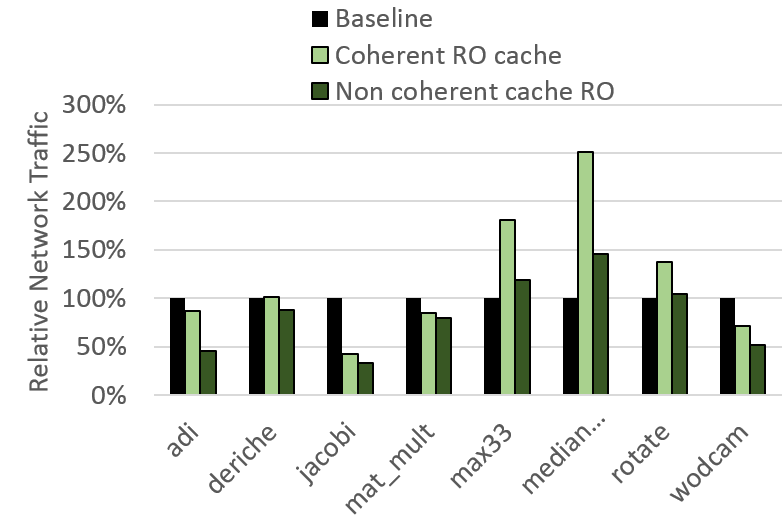
\includegraphics[width=9cm]{./images/resultIncoherent.png}
    \caption{Network traffic variation for coherent and non coherent RO cache}
    \label{resultIncoherent}
\end{figure}

\section{Related Works}

\textbf{Locality Optimization :} 

\subsection{Coherence Optimization}

\subsection{NVM Technologies}

\section{Conclusion}

In this paper the feasibility and benefits of a specific management of read-only data in the memory organization is studied. A complete workflow in a production compiler and simulator has been proposed, making the solution transparent to the user while achieving significant energy improvements, with no significant performance degradation. This separation increases the cache efficiency of the system, and allows specific optimizations for the read-only cache. We have shown that this architectural modification follows the scalability of the shared caches and can be further improved if using non-coherent RO caches. The proposed solution has been validated on a set of image processing applications, but the same methodology could be extended to a larger set of applications. 



\bibliographystyle{ACM-Reference-Format}
\bibliography{cases} 

\end{document}
